\documentclass{jarticle}
\usepackage{abstract}
\usepackage[dvipdfmx]{graphicx}		% eps等図を取り込むためのマクロ

\title{LSTMを用いた楽器エフェクタのシミュレータ構築} %タイトル
\author{氏本 大智}% 報告者
\adviser{長谷 芳樹}% 指導教官

%%平成29年度よりヘッダはwebでpost時に自動で付けるよう変更
% \kind{最終}%
%\kind{中間}%
%\year{28}% 年度
%\num{10}% No.
\thispagestyle{empty}
\pagestyle{empty}

\begin{document}%
\maketitle % タイトルページの出力

\section{はじめに}%
現在,従来はアナログ回路で構成されていた音響機器がディジタル技術でシミュレートされ,ソフトウェアとして実現される場面が多くなっている.音響特性のシミュレート技術も進歩し,数々のシミュレータが開発されている.シミュレートには専用のハードが必要になるケースが多く,ソフトウェア単体で動作するシステムは未だ実用化されていない.

本研究では,ニューラルネットワークの手法を使用し,PCとオーディオインターフェース等の録音機器のみで動作し,エフェクタへの入出力音を入れるだけで音響フィルタを手軽にシミュレートできる,音響フィルタのシミュレータの構築を目的としている.

\section{RNN:Recurrent Neural Network}
通常のニューラルネットワークは時系列データを扱うことができず,時間の概念をニューラルネットワークに取り入れるには,過去の状態をモデル内で保持する必要がある.RNNは,出力を次のステップに入力として渡すことにより,過去の状態が保持され,時系列データを利用できる.\cite{RNN}

今回の研究では,RNNの入出力ゲートを拡張しより長期依存情報をの学習が可能であり,汎用性が高いLSTM(Long Short-Term Memory)を使用する.

\section{実験方法}
\subsection{教師データ作成}
学習に使用する教師データを作成した.
教師データは,110 ms の音声データ (wave ファイル) を入力側と出力側をそれぞれ用意し,それら 1 対を 1 つのデータセットとして扱った.

入力側音声データには,ギターの原音を使用した.サンプリング周波数を48000 Hz,量子分解能を16 bitに設定し,音域,弦を弾く強さ,単音か和音かを無作為に演奏したデータを50 秒分用意した.

出力側データには,用意した入力側音声データをギター用歪みエフェクタの一種であるBOSS DS-1に通したものを使用する.
本研究で使用した録音環境を図1に示す.

\begin{figure}[htbp]
 \begin{center}
  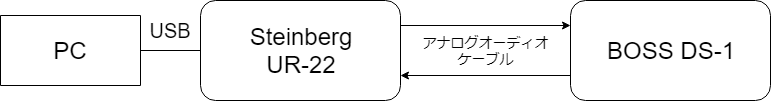
\includegraphics[width=80mm]{env.png}
 \end{center}
 \caption{出力側教師データ録音環境構成図}
 \label{fig:one}
\end{figure}

%\begin{figure}[htbp]
% \begin{center}
%  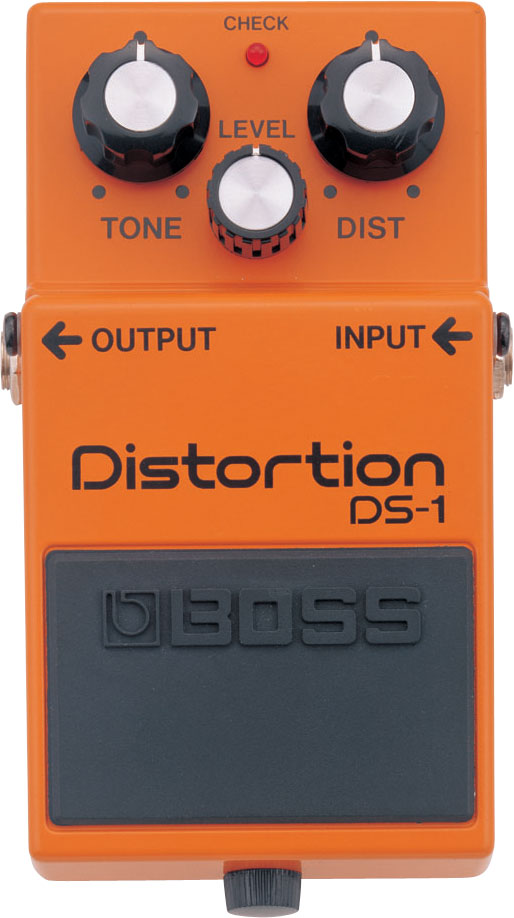
\includegraphics[width=10mm]{ds1.jpg}
% \end{center}
% \caption{BOSS DS-1}
% \label{fig:one}
%\end{figure}

DS-1は,DIST,TONE,LEVELの3つのつまみを持つ.つまみの分解能を,1~9の9段階で定義し,DIST,TONEのつまみを5 パターンの位置に合わせ,データを用意した.

\subsection{学習}

学習モデルにはLSTMを使用し,構成は,input units=64,hidden units=64,output units=1とした.モデル構成図を図2に示す.

\begin{figure}[htbp]
 \begin{center}
  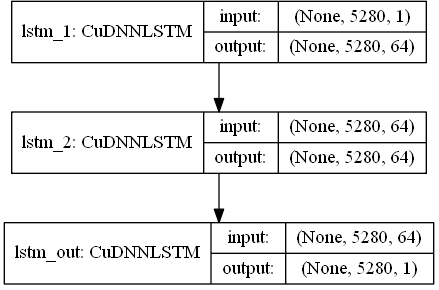
\includegraphics[width=60mm]{model.png}
 \end{center}
 \caption{モデル構成図}
 \label{fig:one}
\end{figure}

LSTM は, 入力データ長と同じ長さの出力が得られるが,今回作成したモデルでは,出力された 110 ms の音声データの 末尾 10 ms を最終出力として使う.
推論の際には,入力側音声データを 10 ms ずつずらしながらモデルを適用 することで完全な出力を整形する.
これにより,出力のすべてが 100 ms の依存情報を得られる.

%\begin{figure}[htbp]
% \begin{center}
%  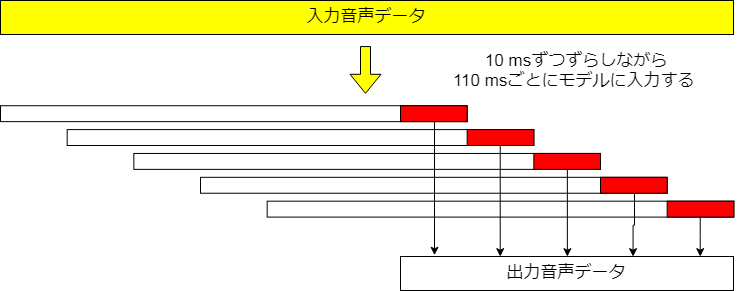
\includegraphics[width=80mm]{suiron.png}
% \end{center}
% \caption{推論イメージ図}
% \label{fig:one}
%\end{figure}

\subsection{評価実験}
学習に使用していないギター音声データを,DS-1と実験3.2で得た学習済みモデルに入力し,DS-1から出力された音声データと,モデルから出力された音声データの出力波形概形,周波数スペクトルを比較した.

\subsection{推論にかかる時間の測定}
5秒の音源を学習済みモデルに入力し,推論された音源が出力されるまでの時間を測定を行った.

\section{結果}
ここでは,実験を行った5パターンのうち,DIST,TONEのつまみを中央の位置にしたものの結果のみを示す.

\subsection{学習結果}
構築したモデルを使用し,16サンプルを1ステップ,100ステップを1Epochとし,100Epochsの計算を行った.学習の際に算出された,教師データとテストデータでの損失算出結果を比較したグラフを図3に示す.
Epochsを重ねるごとに教師データ,テストデータ共に損失は減少しているため,学習により平均二乗誤差を小さくすることに成功している.

\begin{figure}[htbp]
 \begin{center}
  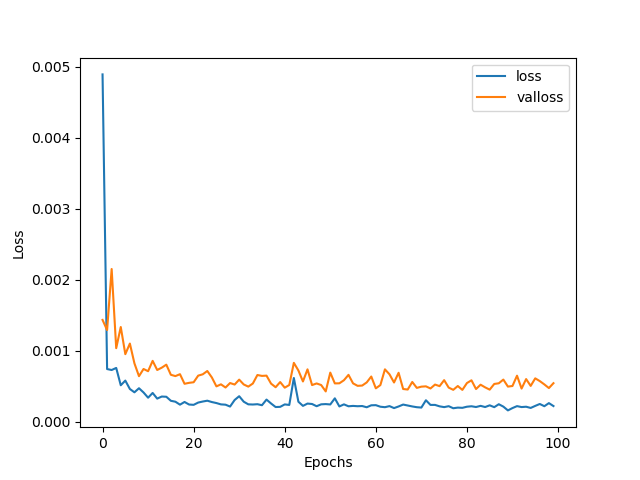
\includegraphics[width=55mm]{gain5_loss_hikaku.png}
 \end{center}
 \caption{損失比較図}
 \label{fig:one}
\end{figure}

\subsection{出力波形比較}
DS-1からの出力音声データと学習済みモデルの出力音声データの波形の概形を比較した.出力波形を図4に示す.概ね教師信号に追従した波形を出力していることがわかる.

\begin{figure}[htbp]
 \begin{center}
  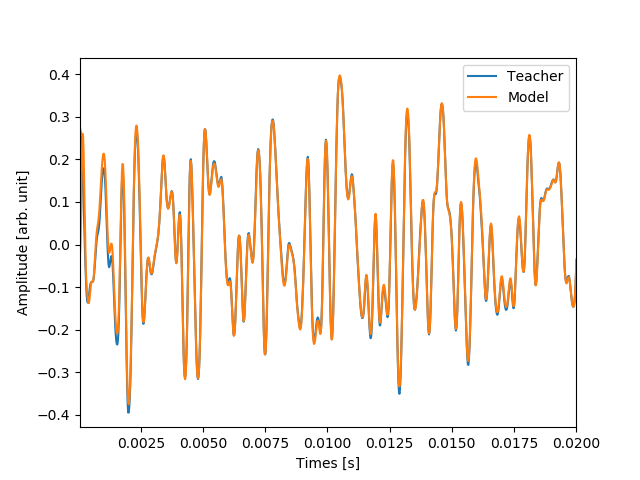
\includegraphics[width=55mm]{gain5_output_hikaku.png}
 \end{center}
 \caption{出力波形比較図}
 \label{fig:one}
\end{figure}

\newpage
\subsection{スペクトル分析}
DS-1からの出力音声データと学習済みモデルの出力音声データにフーリエ変換を行い,周波数スペクトルを比較した.解析結果を図5に示す.低音域は高い再現度を実現しているが,6000 Hz以降の再現度が著しく低下していることがわかる.

\begin{figure}[htbp]
 \begin{center}
  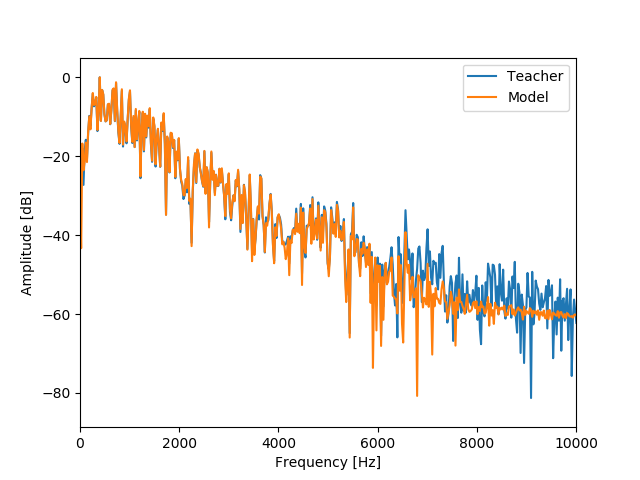
\includegraphics[width=55mm]{gain5_fft_hikaku.png}
 \end{center}
 \caption{スペクトル波形比較}
 \label{fig:one}
\end{figure}

\subsection{推論にかかる時間の測定}

5秒間の音源をモデルに入力し,出力が保存されるまでの時間を5回測定し,平均を算出した.測定結果を表1に示す.
入力音源の時間長の3倍以上の時間がかかっていることがわかる.

\begin{table}[htbp]
  \begin{center}
  \caption{推論にかかる時間測定結果}
  \begin{tabular}{c|c} \hline
    回数&測定時間[s]\\ \hline
    1&17.785 \\
    2&17.956 \\
    3&17.683 \\
    4&17.580 \\
    5&17.854 \\ \hline
    平均&17.772\\ \hline
  \end{tabular}
  \end{center}
\end{table}

\section{考察}
本研究では,PCのみで動作するシミュレータを構築し,エフェクタへの入出力音を用意し学習させることで,ある程度の精度が得られることを実証した.

今後の課題としては,人間の耳で聴取実験を行い,より細かくシミュレータを評価する必要がある.また,ギター演奏の未経験者と経験者では,実験結果に差異が表れるかを明らかにする必要もある.

\begin{thebibliography}{99}%参考文献
\bibitem{RNN}
  巣籠 悠輔 : ``紹介ディープラーニング'', マイナビ出版, pp209-250(2017).
\end{thebibliography}

\end{document}
